\documentclass[a4paper,11pt,bibliography=totoc,listof=totoc,headinclude=true,cleardoublepage=empty]{article}

\usepackage[a4paper,lmargin={3.5cm},rmargin={3.5cm},
tmargin={3.5cm},bmargin = {3.5cm}]{geometry}
\usepackage[utf8]{inputenc}

\usepackage{ifthen}
\usepackage{color}
\usepackage[usenames,dvipsnames]{xcolor}
\usepackage{amsmath,amsthm,amssymb,amsfonts}
\usepackage{tabularx}
\usepackage{mathtools}
\usepackage{graphicx}
\usepackage{psfrag}
\usepackage{multirow}
\usepackage{bigdelim}
\usepackage{relsize}
\usepackage[english]{babel}
\usepackage{ucs} 
\usepackage[utf8]{inputenc}
\usepackage{tocloft}
\usepackage{enumitem}
\usepackage{pdfpages}
\usepackage[export]{adjustbox}
\usepackage{wrapfig}
\numberwithin{equation}{section}

%\usepackage[backend=biber, style=alphabetic ]{biblatex}

\usepackage[sort&compress]{natbib}
%\addbibresource{references.bib}


\author{Simon Mitterhofer}

\DeclareMathOperator*{\esssup}{ess\,sup}
\DeclareMathOperator{\sech}{sech}
\renewcommand{\epsilon}{\varepsilon}
\newcommand{\R}{\mathbb{R}}
\newcommand{\SP}[2]{\langle #1,#2\rangle}

\usepackage[unicode,colorlinks=true,linkcolor=black,pagebackref=false]{hyperref}

\addto\captionsenglish{\renewcommand*\contentsname{Table of Contents}}
\renewcommand{\cftsecleader}{\cftdotfill{\cftdotsep}}
\pagestyle{plain} 


\definecolor{change}{rgb}{0,.55,.55}

\def\revision#1{{\color{red}#1}}









\begin{document}
\pagenumbering{roman}

\begin{titlepage}
    \begin{minipage}{0.6\textwidth}
        
\includegraphics[height=2cm]{files/TULogo.png}
    \end{minipage}\hfill
    \begin{minipage}{0.4\textwidth}
        \hfill 
\includegraphics[height=2cm]{files/logo-imw.jpg}
    \end{minipage}
    
    \begin{center}  
        \vskip 2cm
        {\LARGE \textbf{Bachelor Thesis}}
    
    
    
        \vskip 2cm
    
        {\huge \bfseries Portfolio Choice:}
        \vskip 5mm
        {\LARGE \bfseries Optimal Investment - Consumption Decision}
        \vskip 2cm
    
    

        {\large carried out for the purpose of obtaining the degree of}
        \vskip 3mm
        {\large Bachelor of Science (BSc),}
        \vskip 3mm
        {\large submitted at TU Wien, Faculty of Mechanical and Industrial Engineering, by}
   
        \vskip 2cm
        {\LARGE\bfseries Simon MITTERHOFER}
        
        \vskip 0.5cm
        {\large Mat.Nr.: 11910595}
        \vskip 2cm
        {\large under the supervision of}
        \vskip 5mm
        {\Large a.o. Univ.Prof. DDr. Thomas Dangl}
        \vskip 5mm
        {\Large Institute of Management Science, E330}
    
  \end{center}
  
  \vfill
  
  \begin{center}
       {\Large Vienna, May 6, 2022}
  \end{center}

  \vspace*{-15mm}
\end{titlepage}


\cleardoublepage


%\section*{Eidesstaatliche Erklärung}
%\addcontentsline{toc}{section}{Eidesstaatliche Erklärung}
\input{sections/II_eidesstaatlicheErklärung}

%\newpage
%\section*{Acknowledgement}
%\addcontentsline{toc}{section}{Acknowledgement}
%%\noindent I would like to thank my cousins (Armin, Manuel, Jonas for their help (R, latex and English).\\

%\noindent I would like to thank my parents for always caring and making it possible for me to study.\\

%\noindent I would like to thank my sister and brothers for motivating me.\\

%\noindent I would like to thank Prof. Dangl for providing the possibility and teaching me.

\newpage
\section*{Abstract}
%\addcontentsline{toc}{section}{Abstract}
In this thesis I study a two period consumption and savings problem of an expected power-utility maximizing agent. In order to determine the optimum of the total expected utility, fundamentals of portfolio management and asset pricing are applied. I discuss the effects of a proportional change in returns, as well as a mean preserving spread on the optimal investment strategy. Also, the connection between the price of the investment and the central asset pricing formula is established. In order to simplify the analysis of the problem, I create a corresponding visualization using R-Shiny, which I also describe.\\

\vspace{2cm}

\noindent
Link to the full version:\\
\url{https://drive.google.com/file/d/187nTTkE5RlMnEnewSotXgIUTd-v08uXS/view?usp=share_link}

\thispagestyle{empty}


\newpage
\tableofcontents

\newpage
\pagenumbering{arabic}
\setcounter{page}{1}
\section{Introduction}
Uncertainty is a fundamental aspect of life. Every day, people are exposed to various risks. The economic and financial spheres in particular are characterized by uncertainty. When making investment or other financial decisions, there is usually no safe way to determine in advance what the value of the final outcome will be. \\
Be it an investment decision on the stock exchange, or a simple purchase decision in the supermarket, no one can look into the future. So there is no other option than to rely on probabilities and approximate estimates.\\

\noindent One way to protect yourselves from unforeseen trends is portfolio diversification. On one hand, you may miss out on some of the potential gain from an asset with rising value, but on the other hand, you are better protected against losses from assets with falling value. The goal of a risk-averse investor is to maximize a portfolio’s risk adjusted return, i.e., to optimize its risk/return tradeoff. In return, you give up part of the expected profit. Therefore, it often makes sense not to spend the entire capital on one asset, but to divide and spread it.\\

\noindent I take the concepts presented in this introductory section mostly from \citep{varian2010intermediate} and \citep{ingersoll1987theory}. Some terms essential for understanding are defined and explained in the Theoretical Framework section.

\bigskip

\subsection{Risky investment}

\noindent In a first scenario, the only available investment is a risky asset. An investor, endowed with a certain capital $K$, must today ($t=0)$ decide how much to spend on an investment portfolio and how much to consume. In order to have consumption tomorrow ($t=1$) the investor has to purchase an investment portfolio today such that the portfolio value tomorrow can be consumed. The amount of capital which is consumed today is referred to as $c_0$, the amount available for consumption tomorrow is $c_{1}$.\\
The portfolio's payoff is not known beforehand. It is assumed that there are $N$ possible states, each is assigned a certain probability $\pi_i$ with $i\in\{1,2\dots,N\}$ and a dividend per invested unit of capital, $d_{1,i}$. The probabilities must sum to 100\% and each payoff must be larger than zero. One unit of investment has a price $p_0$, the total amount of units purchased is denoted by $x$. Thus, the amount available for consumption tomorrow is $c_{1,i} \leq x \cdot d_{1,i}$. In the meantime, there is no other way to receive income at $t=1$, so investing today is the only way to receive consumption tomorrow.\\

\noindent The investor derives utility from consumption. Utility from immediate consumption is assumed iso-elastic (i.e., with constant relative risk aversion $\gamma$):

\begin{equation} \label{eqn:isoelastic}
    u(c) = \left\{ \begin{matrix}
                \frac{c^{1-\gamma}-1}{1-\gamma} & \text{if } \gamma \neq 1 , \\
                \ln(c) & \text{if } \gamma = 1.
            \end{matrix}\right.
\end{equation}

\bigskip

\noindent Since future consumption $c_1$ is uncertain, the investor seeks to maximize expected utility, which he/she determines in a time-separable way as 

\begin{equation}\label{eqn:Zielfunktion}
    U = u(c_0) + \beta \cdot \sum_{i=1}^{N} \pi_i \cdot u(c_{1,i})
\end{equation}

\smallskip

\noindent where

\begin{equation}
    \begin{matrix*}[r]
        c_0, c_{1,i} & > & 0,\\
        \beta & \leq & 1,\\
        \gamma & > & 0.
    \end{matrix*}
\end{equation}

\bigskip

\noindent In order to express the investor's time preference the discount factor $\beta$ is introduced. It can be chosen according to the weight the investor places on the utility received tomorrow compared to today.\\
The utility at $t = 1$ is stochastic. Expected utility can be calculated as the sum of the resulting utility in each state, each multiplied by the probability of its occurrence and the discount factor $\beta$.\\

\noindent Ultimately, the investor seeks to maximize the utility function \eqref{eqn:Zielfunktion} with the following constraints:

\begin{equation}\label{eq:scenario1_constraints}
    \begin{matrix*}[l]
        c_0 & = & K - x \cdot p_0, \\
        c_{1,i} & = & x \cdot d_{1,i},\\
        x & \geq & 0.
    \end{matrix*}
\end{equation}


\bigskip

\subsection{Risky and riskless investment}

\noindent In another scenario, it is assumed that the investor has an additional option to receive income tomorrow: a riskless investment. \\
One unit of the riskless investment has a price of $b_0$ and the quantity of riskless units purchased is denoted by $y$. The investor receives a fixed payment of $1$ per unit in each state at $t=1$. So total consumption tomorrow  is the sum of a risky component $x \cdot d_{1,i}$ (the dividend) and a riskless component $y \cdot 1$ (savings in a riskless savings account). \\

\noindent The utility function to be maximized remains the same as in the first scenario, but there are new constraints:

\begin{equation}\label{eq:scenario2_constraints}
    \begin{matrix*}[l]
        c_0 & = & K - x \cdot p_0 - y \cdot b_0, \\
        c_{1,i} & = & x \cdot d_{1,i} + y,\\
        x & \geq & 0,\\
        y & \geq & 0.
    \end{matrix*}
\end{equation}

\bigskip

\noindent The investor seeks to maximize the total expected utility by finding the optimal combination of $x$ and $y$. This also leaves the possibility of not using one of the two investment options at all.

\bigskip

\subsection{Execution}

\noindent The problem was implemented and visualized as an R-Shiny project. This makes it very easy to identify the optimum and the parameters can be selected interactively.

\newpage
\section{Theoretical Framework}
\subsection{Utility}

Although utility was originally introduced by philosophers and economists as a measure of happiness and overall pleasure, in the context of modern economics it is rather used as a tool to model worth or value. Overall this concept is based on the description of preferences and has more of a comparative character \citep[p. 54]{varian2010intermediate}.\\

\noindent A utility function $u(x, y)$ determines the utility which results from the consumption of a certain bundle of goods $(x, y)$ as a numerical value such that a larger number indicates a higher preference. This helps to illustrate the order of preference, however, the numerical magnitude has no intrinsic meaning \citep[p. 90]{nicholson2016microeconomic}. Therefore, it is not possible to say that something gives twice as much utility as something else, as is attempted, for example, in the cardinal utility approach. The focus here is solely on ordering bundles based on the utility generated. To describe choice behavior, ordinal utility is sufficient. For example, if a monotonic transformation such as $f(u) = 2 \cdot u$ is applied to a particular utility function, the value of the utility obtained changes (doubles in this case), but the ordering of our preferences remains the same \citep[p. 56]{nicholson2016microeconomic}.\\

\noindent Nevertheless, it is possible and desirable to search for bundles which have the same utility. All bundles with the same constant utility $u(x_i, y_i) = k$ can be grouped into a set called the level set \citep[p. 59]{varian2010intermediate}. The graphical representation of the level set is called the indifference curve. The consumer is indifferent to all bundles on the indifference curve because they all lead to the same utility level.\\
For different utility levels different indifference curves are displayed. A utility function can be interpreted geometrically as a way of labeling the indifference curves \citep[p. 57]{varian2010intermediate}. A monotonic transformation would consequently mean a relabeling of the indifference curves.

\bigskip

\subsection{Marginal utility}

\noindent Given the utility that a consumer derives from consumption today and tomorrow, $u(c_0, c_1)$, the rate of change in utility as the consumption in one point of time is increased by a small margin $\Delta c_0$, is called marginal utility $MU_{c_0}$.\\
If the additional value is infinitesimally small, one obtains the partial derivative of the utility function, which is equal to the slope of the utility function with respect to $c_0$ while $c_1$ remains fixed \citep[p. 70]{varian2010intermediate}:

\begin{equation}
    MU_{c_0} = \lim_{\Delta c_0 \to 0} \frac{u(c_0 + \Delta c_0, c_1) - u(c_0, c_1)}{\Delta c_0} = \frac{\partial u(c_0, c_1)}{\partial c_0}.
\end{equation}

\bigskip

\noindent The numerical magnitude also has no actual meaning, since it depends on the utility function in question. But it helps to identify where a small increase in immediate consumption would have a large impact on total utility.

\bigskip

\subsection{Expected utility}

If a consumer has to make a choice under uncertainty he/she might take into account the probabilities of different scenarios. The expected utility can then be expressed as a weighted sum of the utility functions in each state, where the weights are given by the probabilities \citep[p. 223]{varian2010intermediate}. A utility function of the form 

\begin{equation}
    U=\sum_i \pi_i u(c_i)
\end{equation}

\bigskip

\noindent is called a von Neumann-Morgenstern utility function.

\bigskip


\subsection{Risk aversion}

Whether an agent is risk-averse or risk-seeking depends on the expected utility function. A risk-averse agent would rather choose a gamble with low uncertainty over a gamble with high uncertainty, even if the expected payoff of the relatively risky gamble is equal or slightly higher compared to the expected payoff of the relatively safe gamble \citep[p. 104]{arrow1996risk}.\\
Conversely, this means that a risk-averse agent is willing to trade risk for some amount of return \citep[p. 122]{pratt1964risk} and the higher the risk aversion, the higher the amount the actor would be willing to pay for insurance.\\

\noindent One way to measure risk aversion is the concavity index or Arrow-Pratt measure of absolute risk aversion \citep[p. 1339]{wakker2008crra}

\begin{equation}
    A(c) = - \dfrac{u''(c)}{u'(c)}.
\end{equation}

\bigskip

\noindent The Arrow-Pratt measure of relative risk aversion is

\begin{equation}
    R(c) = - \dfrac{c \cdot u''(c)}{u'(c)},
\end{equation}

\bigskip

\noindent which, unlike the former, is dimensionless \citep[p. 363]{simon1994mathematics}. Relative risk aversion \lq\lq is useful in analyzing risks expressed as a proportion of the gamble for example investment rates of return" \citep[p. 39]{ingersoll1987theory}.

\bigskip



\subsection{Isoelastic utility function}

\noindent To model the utility created by today's consumption and expected utility of tomorrow's consumption (the value of the investor's portfolio at $t=1$) the isoelastic utility function or power utility function (see equation \ref{eqn:isoelastic}) will be applied. \\
This function belongs to the class of hyperbolic absolute risk aversion functions, which are also called linear risk tolerance utility functions. This means that risk tolerance, which is the reciprocal of the absolute risk aversion, is a linear affine function in consumption \citep[p. 39]{ingersoll1987theory}:

\begin{equation}
    T(c) = \dfrac{1}{A(c)} = \dfrac{c}{1-\gamma} + \dfrac{b}{a} = - \dfrac{u'(c)}{u''(c)}.
\end{equation}

\bigskip

\noindent A special property of the power utility function is the constant relative risk aversion:

\begin{equation}
    \begin{split}
        & u'(c) = c^{-\gamma} \\
        & u''(c) = -\gamma \cdot c^{-\gamma -1}
    \end{split}
\end{equation}

\bigskip

\begin{equation}
    R(c) = - \dfrac{c \cdot u''(c)}{u'(c)} = \gamma.
\end{equation}

\bigskip

\noindent The utility function $u(c)$ of a risk-averse agent is increasing, strictly concave and has positive absolute risk aversion \citep[p. 2]{poon2018finance}, provided that $c \geq 0$:

\begin{equation}\label{eq:ut.func.derivatives}
    u'(c) > 0, \quad u''(c) < 0 \quad \text{and} \quad A(c) > 0.
\end{equation}

\bigskip

\noindent Due to the negative second derivative and therefore strictly monotonically decreasing slope the first marginal unit of consumption has the largest impact $\lim_{c \to 0} u'(c) = \infty$. Thus, the so-called INADA-condition is satisfied. At the same time the effect of an additional unit of input converges to zero when an infinite amount of input is used $\lim_{c \to \infty} u'(c) = 0$ \citep[p. 20]{Uzawa1971sectormodel}. This is referred to as \lq\lq saturation effect\lq\lq. \label{INADA}\\

\noindent With the isoelastic utility function an agent's risk behaviour depends on the constant relative risk aversion $\gamma$. If $\gamma$ is positive, then the actor is risk-averse, otherwise they would be risk seeking, $\gamma = 0$ corresponds to risk neutrality.\\

\noindent The case of $\gamma \rightarrow 1$ can be studied using L'Hospital's rule. For this case, the utility function is equal to the logarithmic function.\\

\noindent In applying the utility function, it is assumed that the quantity consumed cannot be less than zero. In fact, as the function approaches zero the utility diverges to minus infinity, if the agent has a risk aversion larger or equal to $1$. The zero-utility of a less risk-averse agent $(0 < \gamma<1)$ equals $u(0) = -\frac{1}{1-\gamma}$. \\
The limit approaching infinity does also depend on the value of relative risk aversion. If $\gamma \leq 1$, then the function diverges, but if $\gamma > 1$, then the value of the utility function converges to 
$\lim_{c \to \infty} u(c) = \frac{1}{\gamma -1}$. \label{isoel.ut.f:limits}


\newpage
\section{Implementation}
The problem visualisation was implemented as an application using the R-Shiny framework, which consists of three components: a user interface object, a server function and a call function. The code for each component can be found in the appendix.\\

\noindent Essentially the \hyperlink{call function}{call function} just specifies which user interface object and server function to call in the Shiny app.

\bigskip

\subsection{User interface}

\noindent The \hyperlink{User interface}{user interface object} consists of three tabs. The default tab shows the description of the problem, similar to the introduction to this thesis.\\

\begin{figure}[h!]
    \centering
    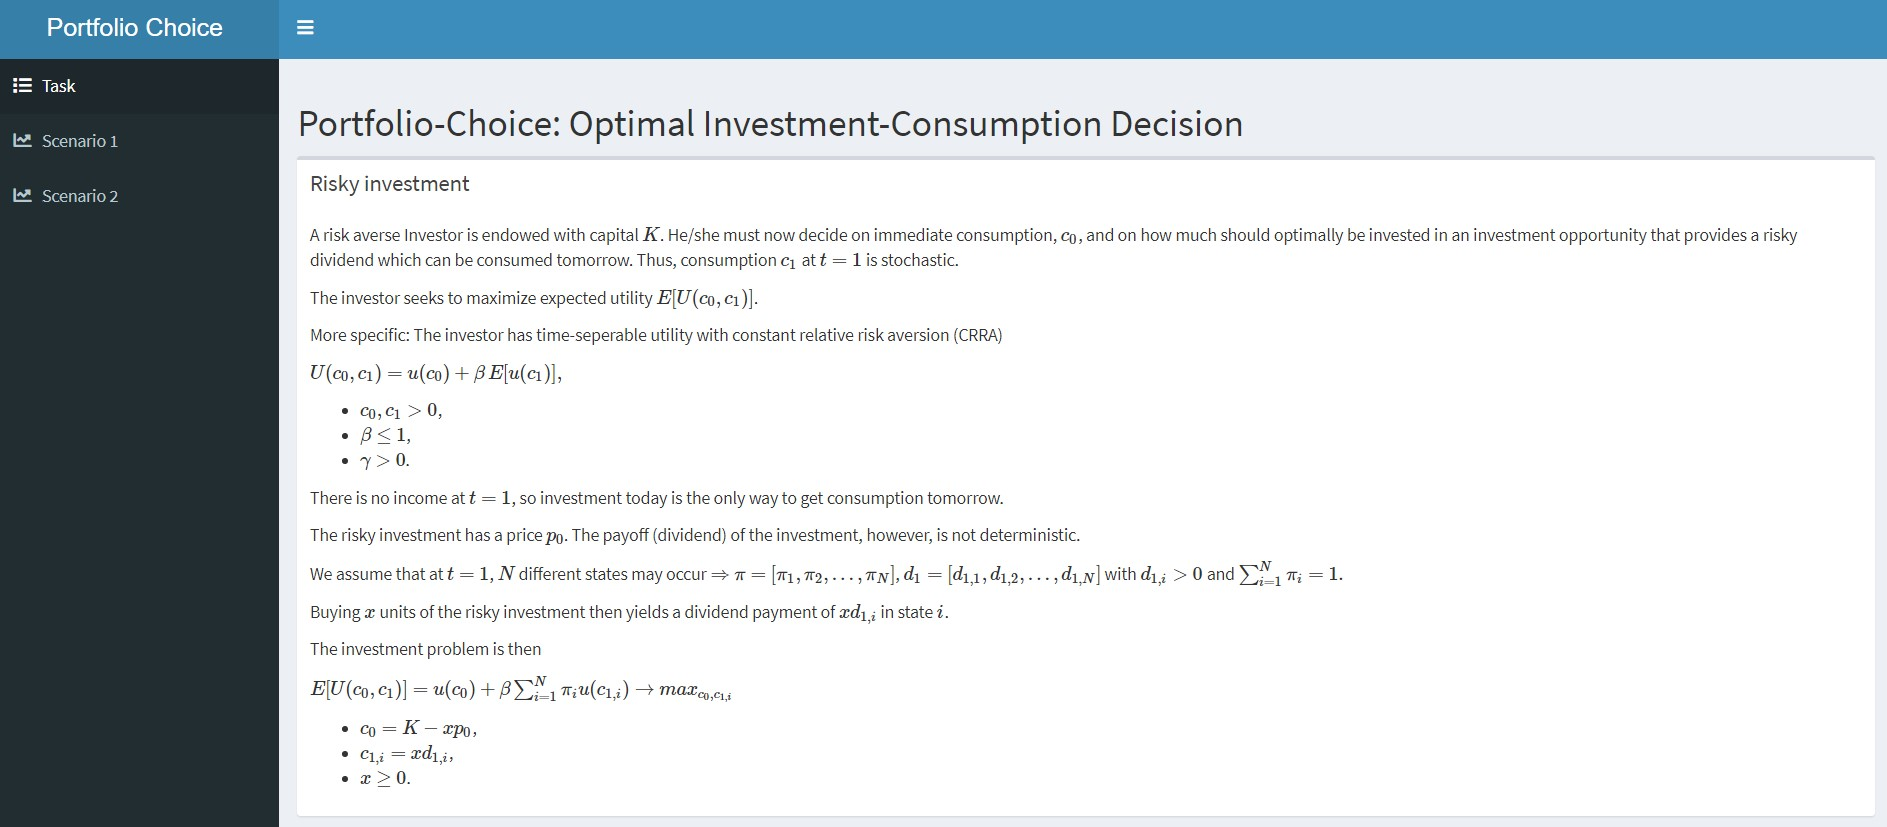
\includegraphics[width=0.7\textwidth, trim = 0 0 0 0,clip]{files/1.1.jpg}
    \caption{Problem description}
\end{figure}

\bigskip

\noindent The second tab is the visualization of the first scenario: The top diagram shows a plot of the utility generated at $t=0$, the expected utility in $t=1$ and the total expected utility.\\
Secondly, a diagram of indifference curves is displayed.\\
Finally, there is a plot of the total expected utility and the marginal utility. \\
All parameters can be set individually by the user. For this purpose, there are sliders on a panel on the left side. There are also two reset buttons, one for the function parameters and one for the investment parameters. At the bottom of the panel, the values of the resulting optimum are displayed.\\
The visualization of scenario 2 is located on the third tab, which is structured analogously.

\bigskip

\subsection{Server function}

\noindent The \hyperlink{Server function}{server function} can be divided into two parts. Up to line 448 the functions for scenario 1 are defined, afterwards the functions for scenario 2. Both parts are once again similar in structure:\\

\noindent First, the function and the default values for the reset buttons are set. In the code, this is done from line 3 to line 79 for scenario 1 and from line 466 to 550 for scenario 2.\\

\noindent From line 80 to 130 and line 551 to 599, respectively, the function comes, which adjusts the probabilities so that the sum always adds up to 100\%.\\

\noindent Between line 131 and 157 and line 600 and 629, respectively, the function parameters and investment specifications are imported and collected into lists for easier processing.\\

\noindent Then, in line 158-187 for scenario 1 and line 630-667 for scenario 2, respectively, the function follows, which maximizes the utility function. It is assumed that the constraints \eqref{eq:scenario1_constraints} and \eqref{eq:scenario2_constraints}, respectively, are binding. In section 4.1 and section 4.2 it is shown that in the optimum this must be true.\\
For simplicity, the utility function is evaluated on a discrete set of points and the maximum can easily be determined. Since the utility function in scenario 1 is one-dimensional, evaluation over a vector is sufficient to find the optimal investment $x^*$. In Scenario 2, the utility function is evaluated over a matrix in order to find the best combination of $x$ and $y$, which is denoted as $(x^*, y^*)$.\\

\noindent Between line 188 and 250 and line 668 and 771, respectively, the charts are generated: For Scenario 1, the first diagram simply consists of the three graphs, total utility, utility at $t=0$ and expected utility at $t=1$, plotted over the amount spent on the risky investment $xp_0$. The diagram for scenario 2 consists of two separate plots. First, the graphs are plotted over $xp_0$ while $yb_0$ remains fixed at $y^*b_0$ and then vice versa.\\

\begin{figure}[h!]
  \centering
  \begin{minipage}[b]{0.44\textwidth}
    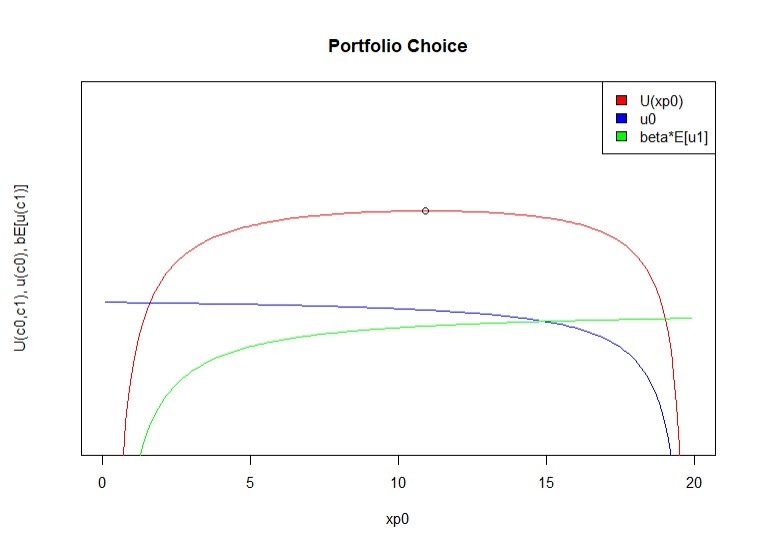
\includegraphics[width=\textwidth, trim = 10 0 30 40,clip]{files/2.1.jpg}
    \caption{Utility, scen. 1}
  \end{minipage}
  \hfill
  \begin{minipage}[b]{0.53\textwidth}
    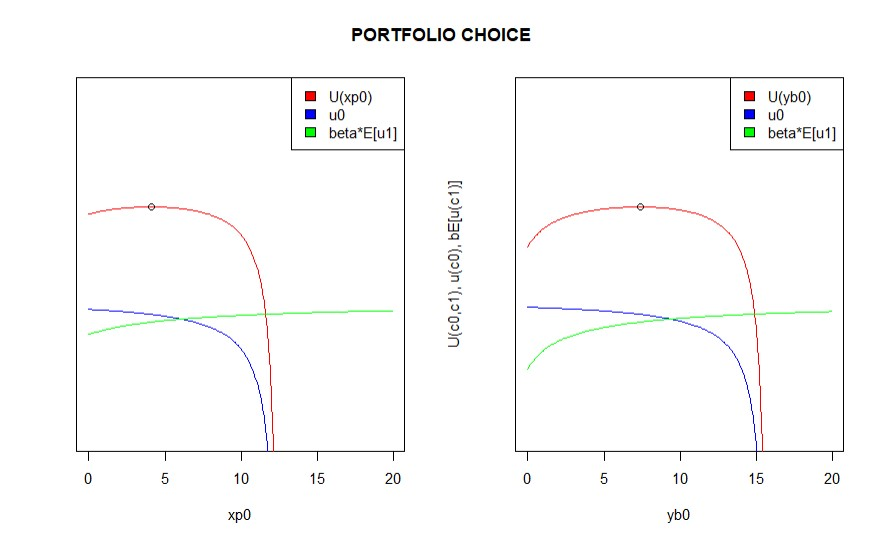
\includegraphics[width=\textwidth, trim = 10 0 20 40,clip]{files/3.1.jpg}
    \caption{Utility, scen. 2}
  \end{minipage}
\end{figure}

\bigskip

\noindent From line 251 to 340 and line 772 to 881, respectively, follows the generation of the plot of indifference curves. The abscissa corresponds to $xp_0$, i.e. the amount of capital spent on the risky investment. The ordinate refers to the amount consumed immediately, $c_0$. For one indifference curve, the constant value is equal to the utility generated in the optimum, which is the maximum possible utility with the given parameters and constraints. Meanwhile, the share of riskless invested capital remains fixed at $y^*b_0$. The other indifference curve can be chosen by the user by adjusting a slider. From then on, things work a little differently for scenario 1 and scenario 2:\\
In scenario 1, the user determines a certain percentage of the original capital. This proportion of capital is then added to (or subtracted from) the originally available capital. The constant value of the indifference curve then corresponds to the maximum utility possible with this newly available capital.\\
In scenario 2, the user determines how much more or less (in percent) is spent on the riskless investment. The budget constraint remains binding. Thus, the amount spent on consumption and the risky investment also changes, and the resulting utility cannot be the optimum. The constant value of the new indifference curve corresponds to the maximum possible utility at the given risk-free expenditure. All points $(xp_0, c_0)$ for which this holds are part of the indifference curve. The legend shows the resulting utilities for the two indifference curves and the amount spent on the riskless investment.\\

\begin{figure}[h!]
  \centering
  \begin{minipage}[b]{0.45\textwidth}
    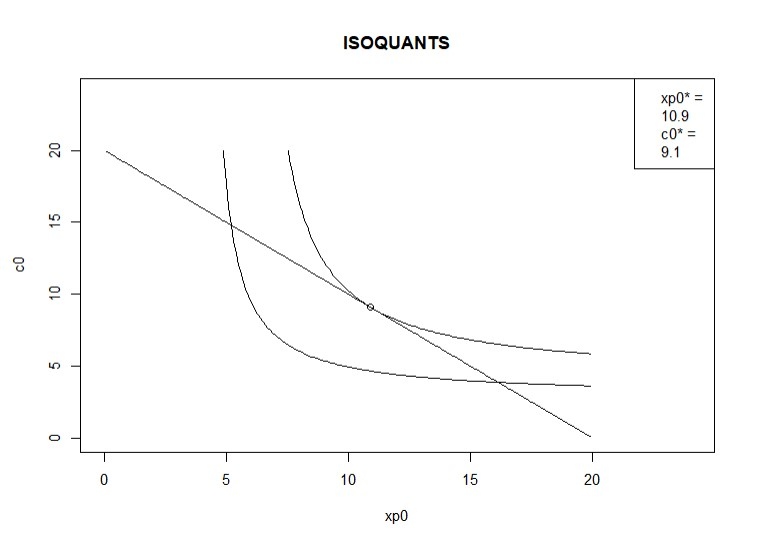
\includegraphics[width=\textwidth, trim = 0 0 0 40,clip]{files/2.2.jpg}
    \caption{Indifference curves, scen. 1}
  \end{minipage}
  \hfill
  \begin{minipage}[b]{0.53\textwidth}
    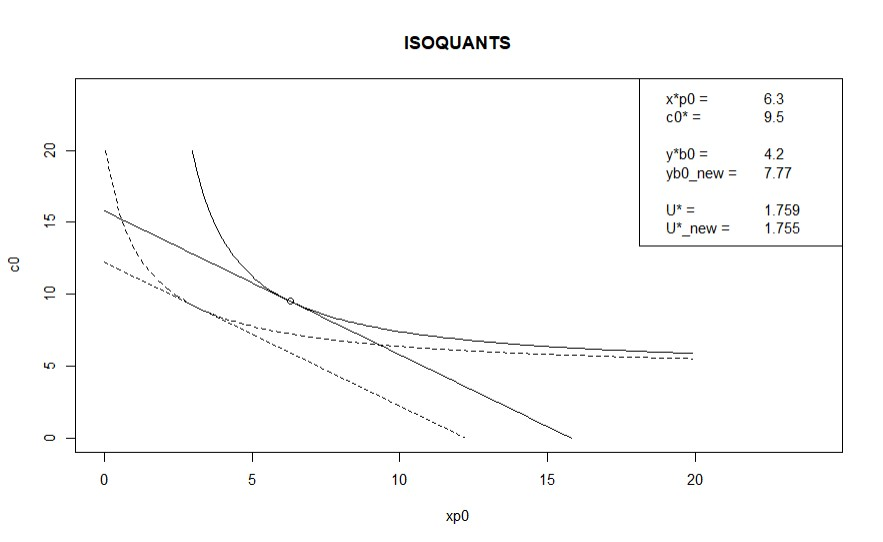
\includegraphics[width=\textwidth, trim = 0 0 0 40,clip]{files/3.2.jpg}
    \caption{Indifference curves, scen. 2}
  \end{minipage}
\end{figure}

\bigskip

\noindent The last diagram is generated between line 341 and 451 for scenario 1 and line 882 and 999. It shows in sub-diagrams the total expected utility plotted over $c_0$, $xp_0$ and $yb_0$, respectively, for scenario 2. The optimum is marked and the marginal utility is shown as a tangent through the optimum.\\

\begin{figure}[h!]
  \centering
  \begin{minipage}[b]{0.47\textwidth}
    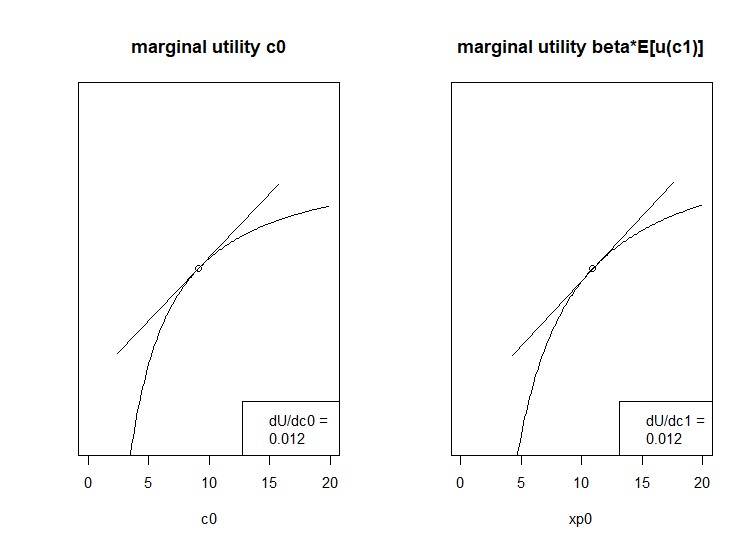
\includegraphics[width=\textwidth, trim = 0 10 0 36,clip]{files/2.3.jpg}
    \caption{Marginal utilities, scen. 1}
  \end{minipage}
  \hfill
  \begin{minipage}[b]{0.51\textwidth}
    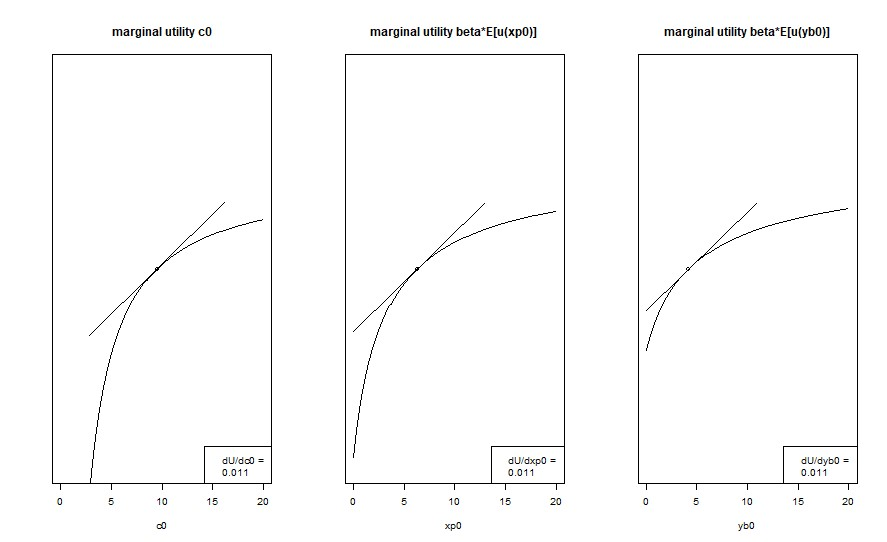
\includegraphics[width=\textwidth, trim = 0 0 0 32,clip]{files/3.3.jpg}
    \caption{Marginal utilities, scen. 2}
  \end{minipage}
\end{figure}

\bigskip

\noindent Finally (lines 452-465 and line 1000-1016, respectively), the function follows which gives the maximum expected utility, the amount consumed immediately and the expenditure on the investments at the optimum.
Small errors may occur, due to the discretization of the domain over which the optimum is evaluated.


\newpage
\section{Model Analysis}
\subsection{Scenario 1}

\noindent The problem to be optimized can be expressed as

\begin{equation}\label{eq:opt.prob1}
\begin{split}
    U(x) &= u(c_0) + \beta \cdot \sum_{i=1}^{N} \pi_i \cdot u(c_{1,i}) \quad \rightarrow \quad \max_{x}\\
    \text{\textit{subject to}} &\\
    c_0 & = K - x \cdot p_0, \\
    c_{1,i} & = x \cdot d_{1,i}, \\
    x & \geq 0.
\end{split}   
\end{equation}

\bigskip

\noindent The Lagrangian associated to this optimization problem is

\begin{equation}\label{eqn:lagr_risky}
\begin{split}
    L(\lambda_i, x, \mu) = u(c_0) + \beta \cdot \sum_{i=1}^{N} & \pi_i \cdot u(c_{1,i}) + \lambda_0 \cdot (K-x \cdot p_0-c_0) + \\ & + \sum_{i=1}^{N} \lambda_i \cdot (x \cdot d_{1,i} - c_{1,i}) + \mu \cdot x.
\end{split}
\end{equation}

\bigskip

\noindent The first order conditions of optimality are formulated as follows:

\begin{minipage}{0.45\textwidth}
    \begin{subequations}\label{eq:lagr1,lambda_0}
    \begin{align}
        \frac{\partial L}{\partial \lambda_0} = K - xp_0 - c_0 & \geq 0 \\
        \lambda_0 & \geq 0 \\
        \lambda_0 \cdot \frac{\partial L}{\partial \lambda_0} & = 0
    \end{align}
    \end{subequations}
\end{minipage}\hfill
\begin{minipage}{0.45\textwidth}
    \begin{subequations}\label{eq:lagr1,lambda_i}
    \begin{align}
        \frac{\partial L}{\partial \lambda_i} = x d_{1,i} - c_{1,i} & \geq 0\\
        \lambda_i & \geq 0\\
        \lambda_i \cdot \frac{\partial L}{\partial \lambda_i} & = 0
    \end{align}
    \end{subequations}    
\end{minipage}\hfill

\bigskip

\begin{minipage}{0.45\textwidth}
    \begin{subequations}\label{eq:lagr1,c_0}
    \begin{align}
        \frac{\partial L}{\partial c_0} = u'(c_0) - \lambda_0 & \leq 0\\
        c_0 & \geq 0 \\
        c_0 \cdot \frac{\partial L}{\partial c_0} & = 0
    \end{align}
    \end{subequations}
\end{minipage}\hfill
\begin{minipage}{0.45\textwidth}
    \begin{subequations}\label{eq:lagr1,c_{1,i}}
    \begin{align}
        \frac{\partial L}{\partial c_{1,i}} = \beta \pi_i u'(c_{1,i}) - \lambda_i & \leq 0\\
        c_{1,i} & \geq 0 \\
        c_{1,i} \cdot \frac{\partial L}{\partial c_{1,i}} & = 0
    \end{align}
    \end{subequations}    
\end{minipage}\hfill

\bigskip

\begin{minipage}{0.45\textwidth}
    \begin{subequations}\label{eq:lagr1,mu}
    \begin{align}
        \frac{\partial L}{\partial \mu} = x & \geq 0\\
        \mu & \geq 0 \\
        \mu \cdot \frac{\partial L}{\partial \mu} & = 0
    \end{align}
    \end{subequations}    
\end{minipage}\hfill
\begin{minipage}{0.45\textwidth}
    \begin{subequations}\label{eq:lagr1,x}
    \begin{align}
        \frac{\partial L}{\partial x} = -\lambda_0 p_0 + \sum_{i=1}^{N} \lambda_i d_{1,i} & \leq 0\\
        x & \geq 0 \\
        x \cdot \frac{\partial L}{\partial x} & = 0
    \end{align}
    \end{subequations}    
\end{minipage}\hfill

\bigskip
\bigskip

\noindent In section \ref{INADA} it has already been stated that the INADA condition is satisfied. Hence, consumption must be larger than zero today $c_0$ and tomorrow $c_{1,i}$. Therefore, the investor will always choose to consume some share of his capital immediately and invest some in order to have consumption tomorrow. \\

\noindent From $c_0$ being strictly positive and the optimality condition \eqref{eq:lagr1,c_0} one can see that 

\begin{equation}\label{eq:opt.cond.lambda_0}
    \lambda_0 = u'(c_0),
\end{equation}

\bigskip

\noindent which is always larger than zero according to equation \eqref{eq:ut.func.derivatives}. Therefore, the first constraint of the optimization problem \eqref{eq:opt.prob1} must be binding (see condition \eqref{eq:lagr1,lambda_0}), which has already been assumed. \\
The Lagrange-multiplier $\lambda_0$ indicates the marginal utility with respect to the available capital $K$: A small increase in capital $\Delta K$ causes a small gain in utility $\Delta u = \lambda_0 \cdot \Delta K$.\\

\noindent Similarly, it can be shown through the optimality condition \eqref{eq:lagr1,c_{1,i}} that

\begin{equation}\label{eq:opt.cond.lambda_i}
    \lambda_i = \beta \pi_i u'(c_{1,i}).
\end{equation}

\bigskip

\noindent The Lagrange-multiplier $\lambda_i$ corresponds to the rate of change of the total utility with respect to $c_{1,i}$ and is again strictly positive, as long as the probability $\pi_i$ is larger than zero. Otherwise this state can be neglected anyway. \\
From condition \eqref{eq:lagr1,lambda_i} follows that also the second boundary condition of the optimization problem \eqref{eq:opt.prob1} is binding. Therefore, also the number of units of the risky investment $x$ purchased by the investor is strictly positive. The Lagrange-multiplier $\mu$ must be zero according to condition \eqref{eq:lagr1,mu}.\\
Furthermore, condition \eqref{eq:lagr1,x} with $x > 0$ leads to

\begin{equation}
    -\lambda_0 p_0 + \sum_{i=1}^{N} \lambda_i d_{1,i} = 0.
\end{equation}

\bigskip

\noindent Applying the equations \eqref{eq:opt.cond.lambda_0} and \eqref{eq:opt.cond.lambda_i} one ultimately gets

\begin{equation}\label{eq:result1}
\begin{split}
    u'(c_0) p_0 & = \beta \sum_{i=1}^{N} \pi_i u'(c_{1,i}) d_{1,i},\\
    c_0 & = K - x p_0,\\
    c_{1,i} & = x d_{1,i}, \quad \forall i.
\end{split}
\end{equation}

\bigskip

\noindent Thus, the optimal investment and consumption strategy is determined by the marginal utility of consumption. Today's consumption is a function of tomorrow's payoffs, state probabilities, the price and the discount factor \citep{dangl2021notes}. \\

\noindent Considering the derivative of the utility function $u'(c) = c^{-\gamma}$, it is possible to transform equation \eqref{eq:result1} as follows:

\begin{equation}\label{eq:spendings-ratio1}
\begin{split}
    &c_0^{-\gamma}p_0 = \beta \sum_{i=1}^{N} \pi_i (c_{1,i})^{-\gamma} d_{1,i}\\
    &\Rightarrow \quad c_0^{-\gamma} = \beta \sum_{i=1}^{N} \pi_i (xd_{1,i})^{-\gamma} \frac{d_{1,i}}{p_0}\\
    &\Rightarrow \quad \bigg( \frac{c_0}{xp_0} \bigg)^{-\gamma} = \beta p_0^{\gamma-1} \sum_{i=1}^{N} \pi_i d_{1,i}^{1-\gamma}\\
    &\Rightarrow \quad \frac{xp_0}{c_0} = \beta^{\frac{1}{\gamma}} p_0^{1- \frac{1}{\gamma}} \bigg( \sum_{i=1}^{N} \pi_i d_{1,i}^{1-\gamma} \bigg) ^{\frac{1}{\gamma}}
\end{split}
\end{equation}

\bigskip

\noindent Hence, the ratio of capital spent on the investment and consumed immediately $\frac{xp_0}{c_0}$ is independent of the amount of initial capital, $K$, and does only depend on the discount factor, the price, the state probabilities and tomorrow's payoffs of the investment.\\

\noindent A smaller discount factor $\beta$ causes the investor to invest less into tomorrow, due to the smaller weight placed on the utility gathered at $t=1$.\\

\noindent The relation between the price $p_0$ and the spending ratio $\frac{xp_0}{c_0}$ depends on the constant relative risk aversion $\gamma$.\\
For $\gamma = 1$ the spending-proportion is independent of the price. A less risk averse agent ($0 < \gamma < 1$) responds to a higher price by spending less on the investment. An investor with higher relative risk aversion ($\gamma > 1$) responds to a higher price by investing more and consuming less.\\
The infinitely risk averse agent would always purchase the same number of investment units $x$, i.e., the spending-ratio is directly proportional to the price $p_0$.\\

\noindent In order to model the influence of a dividend change, the dividends in each state are multiplied by a factor $k$:

\begin{equation*}
    d_{1,i} = k \cdot \tilde{d}_{1,i}
\end{equation*}

\bigskip

\noindent This results in a multiplication of the expected gross return $E(d_{1,i}/p_0)$ by $k$, as well as the standard deviation. Thus, the higher $k$, the higher the expected gross return. An increase in $k$ affects the investment decision in two ways:

\begin{enumerate}[label=(\alph*)]
    \item With higher return from investment, there is an incentive to consume less today in order to profit more from the higher return.
    \item With higher return from investment, there is also an incentive to consume more today, because a lower investment is sufficient to have enough consumption tomorrow \citep{dangl2021notes}.
\end{enumerate}

\noindent After substitution in equation \eqref{eq:spendings-ratio1} the factor $k$ can be separated and it can be seen that the spending ratio $\frac{xp_0}{c_0}$ is proportional to $k^{\frac{1}{\gamma}-1}$.

\begin{equation}
\begin{split}
    \frac{xp_0}{c_0} = \beta^{\frac{1}{\gamma}} \cdot p_0^{1- \frac{1}{\gamma}} \cdot & \bigg( \sum_{i=1}^{N} \pi_i \tilde{d}_{1,i}^{1-\gamma} \bigg) ^{\frac{1}{\gamma}} \cdot k^{\frac{1}{\gamma}-1}\\
    & \\
    \Rightarrow & \quad \frac{xp_0}{c_0} \sim k^{\frac{1}{\gamma}-1}
\end{split}
\end{equation}

\bigskip

\noindent When risk aversion is low ($0<\gamma<1$), an increase in dividends has the same effect as a price cut, because both are an increase in gross return: the investor will spend more on the investment and consume less immediately. Effect (a) is dominant.\\

\noindent Equally, when risk aversion is high ($\gamma>1$), an increase in gross return causes the spending ratio to decrease and more is consumed immediately. Now effect (b) is dominating.\\

\noindent At $\gamma = 1$, the investor is called "myopic" \citep{dangl2021notes}. In this case the investment decision is independent of the expected returns, as well as the price $p_0$.

\bigskip

\begin{figure}[h!]
    \centering
    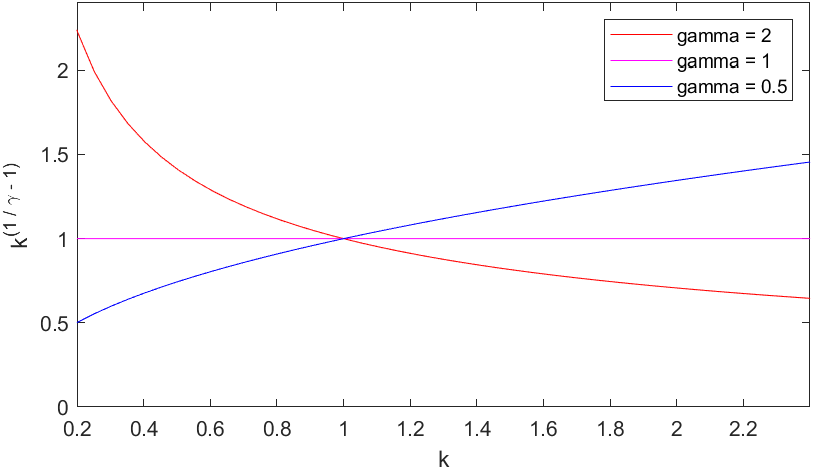
\includegraphics[width=0.7\textwidth]{files/matlab - spending_ratio-k-graph.png}\label{fig:k-spend_ratio}
    \caption{Effect of factor k on the spendings ratio}
\end{figure}

\bigskip

\noindent However, investment behavior is not only determined by the magnitude of the dividends, but also by their variance. I want to illustrate this effect, which is referred to as "mean preserving spread" \citep{rothschild1970mps}, with a simplified model with only two states at $t=1$, $d_{1,1} \leq d_{1,2}$.\\
The probability of occurrence of the two states shall be equal $\pi_1 = \pi_2 = 0.5$. The dividends in each state are chosen such that the expected return $\sum_{i=1}^{2} \pi_i d_{1,i}$ remains constant at $1$. The abscissa is to describe the spread $s$ of the dividends, modelled as $1-\frac{d_{1,1}}{d_{1,2}}$:

\begin{equation*}
\begin{split}
    d_{1,1} &= \frac{2-2s}{2-s}\\
    d_{1,2} &= \frac{2}{2-s}
\end{split}
\end{equation*}

\bigskip

\noindent At $s=0$ the dividends $d_{1,1}$ and $d_{1,2}$ are equal, there is no spread. As $s$ approaches $1$, $d_{1,1}$ converges towards $0$, while the expected return must remain constant. Therefore, $d_{1,2}$ approaches $2$. At $s=1$ the spread is at its maximum. Meanwhile, $\beta$ and $p_0$ are both fixed at a value of $1$.\\


\begin{figure}[h!]
    \centering
    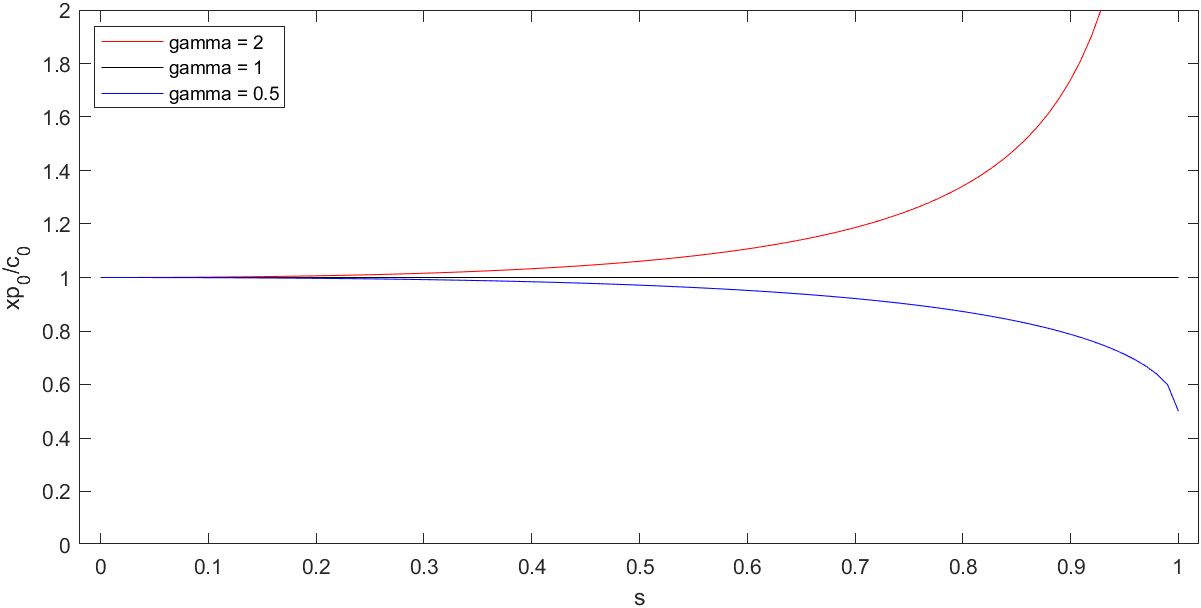
\includegraphics[width=0.7\textwidth]{files/matlab - mean preserving spread s.png}\label{fig:s-dividends-spread}
    \caption{Effect of mean preserving spread on the spending ratio}
\end{figure}

\bigskip

\noindent This diagram shows that the influence of \lq\lq mean preserving spread" depends on the relative risk aversion $\gamma$:\\
At $\gamma = 1$, the spending ratio once again remains unaffected by the dividends.\\
An investor with a strong risk aversion $(\gamma>1)$ reacts to an increase in dividend spread with a larger investment portion. This is due to the fact, that the highly risk averse investor fears to be left with little or even no consumption at $t=1$. A larger investment should offset this risk.\\
Conversely, when risk aversion is lower than one, a large dividend spread results in more immediate consumption. The slightly risk averse investor does not consider it necessary to hedge against the risk of low returns because the minimum utility is limited (see page \pageref{isoel.ut.f:limits}). More of the capital is spent on immediate consumption because its resulting utility is certain.


\vspace{10mm}

\noindent An alternative approach to determine the optimum is by substitution of $c_0$ with $K-xp_0$ in the original optimization problem \eqref{eq:opt.prob1}:

\begin{equation}
    f(x) = u(K - xp_0) + \beta \sum_{i=1}^{N} \pi_i u(c_{1,i}).
\end{equation}

\bigskip

\noindent The model, which originally was a model in $c_0$ and uncertain $c_1$, can now be described with a one-dimensional function in $x$. The optimum can be found through differentiation and solving for the maximum:

\begin{equation}
    \frac{d}{dx} f(x) = -p_0 u'(K - xp_0) + \beta \sum_{i=1}^{N} \pi_i u'(c_{1,i}) d_{1,i} = 0
\end{equation}

\bigskip

\noindent This leads to the same result as obtained in equation \eqref{eq:result1}. Since the objective function is globally concave in $x$ and $y$ and all constraints are linear in these investment decisions, 2nd-order optimality conditions are satisfied, i.e., the determined candidate $(x^*,y^*)$ maximizes the investors utility \citep[p. 131]{dangl2022bwopt}.\\

\noindent It is noticeable that by taking the derivative with respect to $xp_0$ instead of $x$, one side of the equation yields exactly the derivative of the total utility function $U(c_0, c_1)$ from equation \eqref{eq:opt.prob1} with respect to $c_0$:

\begin{equation}
    \frac{\partial U}{\partial c_0} = u'(c_0) = MU_{c_0}
\end{equation}

\bigskip

\noindent The other side of the equation equals the derivative of the total utility with respect to $xp_0$:

\begin{equation}
    \frac{\partial U}{\partial (xp_0)} = \beta \sum_{i=1}^{N} \pi_i u'(c_{1,i}) \frac{d_{1,i}}{p_0} = MU_{xp_0}
\end{equation}

\bigskip

\noindent Thus, the marginal utilities with respect to $c_0$ and $xp_0$ must be equal, i.e., the increase in utility caused by an additional unit of capital must be the same, whether it is consumed immediately or invested.\\
Otherwise it would be possible to gain utility by simply transferring a small amount of capital from the investment option with lower marginal utility to the asset with higher marginal utility:

\begin{align*}
    \text{if} & \quad MU_{c_0} >(<) MU_{xp0}:\\
    \\
    \Delta U & \cong -MU_{xp0} \cdot \Delta K + MU_{c_0} \cdot \Delta K\\
    & = \Delta K \cdot (MU_{c_0} - MU_{xp0}) >(<) 0. 
\end{align*}

\bigskip

\noindent This would be contrary to the fundamental properties of an optimum. Therefore, in the maximum point the marginal utilities with respect to $c_0$ and $xp_0$ must be equal.

\vspace{10mm}

\noindent Other interesting aspects of this problem can be determined by rearranging equation \eqref{eq:result1} as follows:

\begin{equation}\label{eq:pricing_eq1}
    p_0 = \sum_{i=1}^{N} \pi_i \beta \frac{u'(c_{1,i})}{u'(c_0)} d_{1,i}
\end{equation}

\bigskip

\noindent This equation is the "central asset pricing formula" 
\citep[p. 6]{cochrane2001asset}. The right side is called the expected discounted value of the asset's payoff. If the price does not match this function of payoffs, there exists a change in the investor’s investment strategy such that the the associated change in consumption would improve the investor’s total expected utility. The term

\begin{equation}\label{eq:stochastic_disc_fac}
    m_i = \beta \frac{u'(c_{1,i})}{u'(c_0)}
\end{equation}

\bigskip

\noindent is called the stochastic discount factor. It can be thought of as a weight placed on the different possible states, similar to the discount factor $\beta$, but state dependent, regarding differences in (marginal) utility.\\
For example, if there was a risk neutral investor ($\gamma = 0$), then the stochastic discount factor would be equal to $\beta$:

\begin{equation*}
    u'(c) = 1 \quad \Rightarrow \quad m_i = \beta.
\end{equation*}

\bigskip

\noindent Therefore, the investor's equilibrium price exactly matches the discounted expected dividend

\begin{equation*}
    p_0(\gamma = 0) =  \beta \sum_{i=1}^{N} \pi_i d_{1,i}.
\end{equation*}

\bigskip

\noindent A risk averse agent has different stochastic discount factors $m_i$ for different states. For a high level of consumption, tomorrow's marginal utility is low (due to saturation). Thus, a lower weight is placed on the states with higher dividends. States with a relatively low level of consumption have a disproportionately high weight \citep{dangl2021notes}.\\

\noindent In other words, to a risk averse investor, the probability of a state $i$ appears higher than it actually is if the dividend $d_{1,i}$ is lower compared to the others. Conversely, states with higher dividend receive lower weight.







\newpage
\subsection{Scenario 2}

\noindent Compared to scenario 1, now the investor has a second option to invest his capital in order to receive consumption at t=1, a riskless investment. Therefore, there are additions in the constraints, the objective function of the optimization problem remains the same:

\begin{equation}\label{eq:opt.prob2}
\begin{split}
    U(x, y) &= u(c_0) + \beta \cdot \sum_{i=1}^{N} \pi_i \cdot u(c_{1,i}) \quad \rightarrow \quad \max_{x, y}\\
    \text{subject to} &\\
    c_0 & = K - x \cdot p_0 - y \cdot b_0 \\
    c_{1,i} & = x \cdot d_{1,i} + y \cdot 1 \\
    x & \geq 0\\
    y & \geq 0
\end{split}   
\end{equation}

\bigskip

\noindent The Lagrangian, which belongs to this optimization problem is

\begin{multline}\label{eq:lagr_riskless}
    L(\lambda_i, x, \mu_x, y, \mu_y) = u(c_0) + \beta \cdot \sum_{i=1}^{N} \pi_i \cdot u(c_{1,i}) + \lambda_0 \cdot (K-x p_0 - y b_0 -c_0) + \\ + \sum_{i=1}^{N} \lambda_i \cdot (x d_{1,i} + y \cdot 1 - c_{1,i}) + \mu_x \cdot x + \mu_y \cdot y
\end{multline}

\bigskip

\noindent Next, the first order conditions of optimality are formulated:

\begin{minipage}{0.48\textwidth}
    \begin{subequations}\label{eq:lagr2,lambda_0}
    \begin{align}
        \frac{\partial L}{\partial \lambda_0} = K - xp_0 - yb_0 - c_0 & \geq 0 \\
        \lambda_0 & \geq 0 \\
        \lambda_0 \cdot \frac{\partial L}{\partial \lambda_0} & = 0
    \end{align}
    \end{subequations}
\end{minipage}
\begin{minipage}{0.48\textwidth}
    \begin{subequations}\label{eq:lagr2,lambda_i}
    \begin{align}
        \frac{\partial L}{\partial \lambda_i} = x d_{1,i} + y - c_{1,i} & \geq 0\\
        \lambda_i & \geq 0\\
        \lambda_i \cdot \frac{\partial L}{\partial \lambda_i} & = 0
    \end{align}
    \end{subequations}    
\end{minipage}

\bigskip

\begin{minipage}{0.48\textwidth}
    \begin{subequations}\label{eq:lagr2,c_0}
    \begin{align}
        \frac{\partial L}{\partial c_0} = u'(c_0) - \lambda_0 & \leq 0\\
        c_0 & \geq 0 \\
        c_0 \cdot \frac{\partial L}{\partial c_0} & = 0
    \end{align}
    \end{subequations}
\end{minipage}\hfill
\begin{minipage}{0.48\textwidth}
    \begin{subequations}\label{eq:lagr2,c_i}
    \begin{align}
        \frac{\partial L}{\partial c_{1,i}} = \beta \pi_i u'(c_{1,i}) - \lambda_i & \leq 0\\
        c_{1,i} & \geq 0 \\
        c_{1,i} \cdot \frac{\partial L}{\partial c_{1,i}} & = 0
    \end{align}
    \end{subequations}    
\end{minipage}\hfill

\bigskip

\begin{minipage}{0.48\textwidth}
    \begin{subequations}\label{eq:lagr2,mu_x}
    \begin{align}
        \frac{\partial L}{\partial \mu_x} = x & \geq 0\\
        \mu_x & \geq 0 \\
        \mu_x \cdot \frac{\partial L}{\partial \mu_x} & = 0
    \end{align}
    \end{subequations}    
\end{minipage}\hfill
\begin{minipage}{0.48\textwidth}
    \begin{subequations}\label{eq:lagr2,mu_y}
    \begin{align}
        \frac{\partial L}{\partial \mu_y} = y & \geq 0\\
        \mu_y & \geq 0 \\
        \mu_y \cdot \frac{\partial L}{\partial \mu_y} & = 0
    \end{align}
    \end{subequations}    
\end{minipage}\hfill

\bigskip

\begin{minipage}{0.48\textwidth}
    \begin{subequations}\label{eq:lagr2,x}
    \begin{align}
        \frac{\partial L}{\partial x} = -\lambda_0 p_0 + \sum_{i=1}^{N} \lambda_i d_{1,i} & \leq 0\\
        x & \geq 0 \\
        x \cdot \frac{\partial L}{\partial x} & = 0
    \end{align}
    \end{subequations}    
\end{minipage}
\begin{minipage}{0.48\textwidth}
    \begin{subequations}\label{eq:lagr2,y}
    \begin{align}
        \frac{\partial L}{\partial y} = -\lambda_0 b_0 + \sum_{i=1}^{N} \lambda_i & \leq 0\\
        y & \geq 0 \\
        y \cdot \frac{\partial L}{\partial y} & = 0
    \end{align}
    \end{subequations}    
\end{minipage}

\vspace{10mm}

\noindent Again, due to the satisfied INADA condition, $c_0$ and $c_{1,i}$ must be strictly positive. From condition \eqref{eq:lagr2,c_0} and $c_0 > 0$ follows that

\begin{equation}\label{eq:opt.cond.2.lambda_0}
    \lambda_0 = u'(c_0),
\end{equation}

\bigskip

\noindent which is strictly positive as well. $\lambda_0$ is the lagrange multiplier of the budget constraint, i.e., the marginal value of an additional unit of initial wealth. Equation \eqref{eq:opt.cond.2.lambda_0} can be applied to condition \eqref{eq:lagr2,lambda_0} and it can be concluded that the first constraint of the optimization problem \eqref{eq:opt.prob2} is binding, as already assumed.\\
Similarly, from $c_{1,i} > 0$ one can conclude by the condition \eqref{eq:lagr2,c_i} that

\begin{equation}\label{eq:opt.cond.2.lambda_i}
    \lambda_i = \beta \pi_i u'(c_{1,i}) \quad \Rightarrow \quad \dfrac{\lambda_i}{\lambda_0}=m_i \cdot \pi_i.
\end{equation}

\bigskip

\noindent Since $\lambda_i$ is also strictly positive, the condition \eqref{eq:lagr2,lambda_i} can be applied, which leads to the conclusion that also the second boundary condition of the problem \eqref{eq:opt.prob2} must be binding.\\

\noindent It is, however, not immediately clear, whether the investor optimally builds a portfolio from both assets (the riskless and the risky asset) or whether she only uses one of those. The case of no investment is technically also an opportunity, but can be ruled out later. The four cases to be examined are the following:

\begin{align*}
    (I)& \quad   x = 0,\ y = 0      \\
    (II)& \quad   x > 0,\ y = 0     \\
    (III)& \quad   x = 0,\ y > 0    \\
    (IV)& \quad   x > 0,\ y > 0
\end{align*}

\bigskip

\noindent Case $(I)$ can be ruled out, since

\begin{equation*}
    c_{1,i} = x \cdot d_{1,i} + y \cdot 1
\end{equation*}

\bigskip

\noindent is binding and $c_{1,i} > 0$. \\

\noindent In case $(II)$ one has

\begin{equation*}
    c_{1,i} = x \cdot d_{1,i} \qquad \text{and} \qquad c_0 = K - x \cdot p_0.
\end{equation*}

\bigskip

\noindent From condition \eqref{eq:lagr2,mu_x} can be concluded that $\mu_x = 0$. Condition \eqref{eq:lagr2,x} with equations \eqref{eq:opt.cond.2.lambda_0} and \eqref{eq:opt.cond.2.lambda_i} applied leads to

\begin{equation}
    u'(c_0) = \beta \sum_{i=1}^{N} \pi_i u'(c_{1,i}) \frac{d_{1,i}}{p_0}.
\end{equation}

\bigskip

\noindent Since $y=0$, no new conclusions can be drawn from condition \eqref{eq:lagr2,mu_y}. Condition \eqref{eq:lagr2,y} shows that only if $b_0$ is large, i.e. the riskless rate is low, the investor is willing to hold only the risky asset.\\

\noindent Case $(III)$ works similarly. Here one has

\begin{equation*}
    c_{1,i} = y \qquad \text{and} \qquad c_0 = K - y \cdot b_0.
\end{equation*}

\bigskip

\noindent $\mu_y = 0$, due to condition \eqref{eq:lagr2,mu_y}. Conditions \eqref{eq:lagr2,mu_x} leads to no new conclusions. Condition \eqref{eq:lagr2,x} gives that only if $p_0$ is high compared to the dividends the investor will only hold the riskless asset.\\
Through application of equations \eqref{eq:opt.cond.2.lambda_0} and \eqref{eq:opt.cond.2.lambda_i}, one finds that

\begin{equation}
    u'(c_0) = \beta \sum_{i=1}^{N} \pi_i u'(c_{1,i}) \frac{1}{b_0}.
\end{equation}

\bigskip

\noindent Case $(IV)$ is the really interesting case where the prices of both assets are attractive in the sense that the investor optimally builds a portfolio from both.

\begin{equation*}
    c_{1,i} = x d_{1,i} + y \qquad \text{and} \qquad c_0 = K - x p_0 - y b_0.
\end{equation*}

\bigskip

\noindent Conditions \eqref{eq:lagr2,mu_x} and \eqref{eq:lagr2,mu_y} lead to $\mu_x = \mu_y = 0$. The evaluation of conditions \eqref{eq:lagr2,x} and \eqref{eq:lagr2,y} results in

\begin{equation}\label{eq:sol.prob2}
\begin{split}
    u'(c_0) &= \beta \sum_{i=1}^{N} \pi_i u'(c_{1,i}) \frac{d_{1,i}}{p_0}=\\
    &= \beta \sum_{i=1}^{N} \pi_i u'(c_{1,i}) \frac{1}{b_0}.
\end{split}
\end{equation}

\bigskip

\noindent Here, too, it is apparent that each part of this equation corresponds to the derivatives of the total expected utility function \eqref{eq:opt.prob2} with respect to $c_0$, $xp_0$ and $yb_0$, which are the marginal utilities, respectively:

\begin{align*}
    \frac{\partial U}{\partial c_0} &= u'(c_0) = MU_{c_0}, \\
    \frac{\partial U}{\partial (xp_0)} &= \beta \sum_{i=1}^{N} \pi_i u'(c_{1,i}) \frac{d_{1,i}}{p_0} = MU_{xp_0}, \\
    \frac{\partial U}{\partial (yb_0)} &= \beta \sum_{i=1}^{N} \pi_i u'(c_{1,i}) \frac{1}{b_0} = MU_{yb_0}\\
    &\\
    \Rightarrow & \quad MU_{c_0} = MU_{xp_0} = MU_{yb_0}.
\end{align*}

\bigskip

\noindent In case $(IV)$ the marginal utilities must all be equal, such that the investor is indifferent how to invest an additional unit of capital $\Delta K$.\\
In case $(II)$, only $MU_{c_0} = MU_{xp_0}$ is known. However, $MU_{yb_0}$ cannot be larger than $MU_{c_0}$ and $MU_{xp_0}$, because then the investor could gain utility by reallocating invested capital from the risky investment to the riskless investment, but this would contradict the properties of an optimum, as already explained on page 12. \\
$MU_{yb_0}$ can very well be smaller than $MU_{c_0}$ and $MU_{xp_0}$, since there is no capital that could be shifted from the riskless investment to the risky investment and thus, no possible utility gain.\\
The same can be concluded from condition \eqref{eq:lagr2,y} after applying equations \eqref{eq:opt.cond.2.lambda_0} and \eqref{eq:opt.cond.2.lambda_i}. \\

\noindent With no share of capital being invested risklessly, the investor is in the same situation as in scenario 1. Thus, the investment-consumption-ratio can again be described as

\begin{equation}
    \frac{xp_0}{c_0} = \beta^{\frac{1}{\gamma}} \cdot p_0^{1-\frac{1}{\gamma}} \cdot \bigg( \sum_{i=1}^{N} \pi_i d_{1,i}^{1-\gamma} \bigg)^{\frac{1}{\gamma}}.
\end{equation}

\bigskip

\noindent Case $(III)$ works similarly. Here, $MU_{c_0}$ and $MU_{yb_0}$ are equal and $MU_{xp_0}$ must be smaller or equal. This can also be concluded from condition \eqref{eq:lagr2,x}.\\
The relation between the share of capital invested risklessly and consumed immediately is

\begin{equation}
    \frac{yb_0}{c_0} = \beta^{\frac{1}{\gamma}} \cdot b_0^{1-\frac{1}{\gamma}},
\end{equation}

\bigskip

\noindent which is similar to the relation before: The spending ratio only depends on the discount factor $\beta$, the price $b_0$ and the relative risk aversion $\gamma$.

\bigskip

\noindent In order to know which case applies, one can use the observations about marginal utilities: For case $(II)$ to apply $(x > 0,\ y = 0)$, $MU_{yb_0}$ cannot be larger than $MU_{xp_0}$.

\begin{equation*}
\begin{split}
    MU_{yb_0} &\leq MU_{xp_0}\\
    \beta \sum_{i=1}^{N} \pi_i u'(c_{1,i}) \frac{1}{b_0} &\leq \beta \sum_{i=1}^{N} \pi_i u'(c_{1,i}) \frac{d_{1,i}}{p_0}
\end{split}
\end{equation*}

\bigskip

\noindent Also, consumption at $t=1$ is only possible through the return of the risky investment, thus, $c_{1,i} = x \cdot d_{1,i}$. Therefore, one gets

\begin{equation}\label{eq:2xp0b0,y0}
\begin{split}
    \beta \sum_{i=1}^{N} \pi_i u'(xd_{1,i}) \frac{1}{b_0} &\leq \beta \sum_{i=1}^{N} \pi_i u'(xd_{1,i}) \frac{d_{1,i}}{p_0}\\
    &\Leftrightarrow\\
    \frac{p_0}{b_0} &\leq \frac{\sum_{i=1}^{N} \pi_i d_{1,i}^{1-\gamma}}{\sum_{i=1}^{N} \pi_i d_{1,i}^{-\gamma}}.
\end{split}
\end{equation}

\bigskip

\noindent From (4.29a), (4.30a) and (4.32) we see that

\begin{equation*}
\begin{split}
    p_0 &= \sum_{i=1}^N \frac{\lambda_i \cdot d_{1,i}}{\lambda_0} = \sum_{i=1}^N \pi_i \cdot m_i \cdot d_{1,i} = E(md_1),\\
    b_0 &\geq \sum_{i=1}^N \frac{\lambda_i}{\lambda_0} \cdot 1 = E(m).
\end{split}
\end{equation*}

\bigskip
\noindent Since only the risky asset is invested, the stochastic discount factor only prices the risky asset. But the asset pricing formula states that \lq\lq the riskless asset is too expensive\lq\lq.\\
(4.38) can be reformulated in terms of the stochastic discount factor $m_i$:

\begin{equation*}
    \frac{p_0}{b_0} \leq \frac{\sum_{i=1}^{N} \pi_i m_i d_{1,i}}{\sum_{i=1}^{N} \pi_i m_i} = \frac{E(md_1)}{E(m)}.
\end{equation*}

\bigskip

\noindent Similarly, for case $(III)$: Here, $MU_{xp_0}$ cannot be larger than $MU_{yb_0}$. The investor gets consumption at $t=1$ only through the return of the riskless investment, therefore, $c_{1,i} = y$. \\
Again, from (4.29a), (4.30a) and (4.32) we see that

\begin{equation*}
\begin{split}
    p_0 &\geq E(md_1),\\
    b_0 &= E(m).
\end{split}
\end{equation*}

\bigskip
\noindent Now only the riskless asset is priced, since the risky asset is not used. This means that \lq\lq the risky asset is too expensive\lq\lq . It follows that

\begin{equation}\label{eq:2yp0b0,x0}
\begin{split}
    \beta \sum_{i=1}^{N} \pi_i u'(y) \frac{1}{b_0} &\geq \beta \sum_{i=1}^{N} \pi_i u'(y) \frac{d_{1,i}}{p_0}\\
    &\Leftrightarrow\\
    \frac{p_0}{b_0} \geq \frac{\sum_{i=1}^{N} \pi_i d_{1,i}}{\sum_{i=1}^{N} \pi_i} &= \sum_{i=1}^{N} \pi_i d_{1,i} = E(d_1).
\end{split}
\end{equation}

\bigskip

\noindent Thus, it is possible to determine in advance which case applies, based on the prices, tomorrow's payoffs and state probabilities:

\begin{equation*}
\begin{split}
    \text{case } (II)& \qquad \frac{p_0}{b_0} \leq \frac{\sum_{i=1}^{N} \pi_i d_{1,i}^{1-\gamma}}{\sum_{i=1}^{N} \pi_i d_{1,i}^{-\gamma}}\\
    \Rightarrow \quad x>0,\ y = 0&\\
    \text{case } (III)& \qquad \frac{p_0}{b_0} \geq \sum_{i=1}^{N} \pi_i d_{1,i}\\
    \Rightarrow \quad x=0,\ y > 0&\\
    \text{case } (IV)& \qquad \frac{\sum_{i=1}^{N} \pi_i d_{1,i}^{1-\gamma}}{\sum_{i=1}^{N} \pi_i d_{1,i}^{-\gamma}} < \frac{p_0}{b_0} < \sum_{i=1}^{N} \pi_i d_{1,i} \\
    \Rightarrow \quad x > 0,\ y > 0&
\end{split}
\end{equation*}

\bigskip

\noindent In order to find the optimal investment-consumption strategy the investor simply has to determine which case applies. If case $(II)$ or $(III)$ apply, he/she can easily determine the investment-consumption ratio through (4.36), or (4.37), respectively.\\

\smallskip

\noindent At $\gamma = 0$, the statements from equation \eqref{eq:2xp0b0,y0} and \eqref{eq:2yp0b0,x0} are equal, except for the inequality sign. Thus, the risk neutral investor would consider both investments only if the price ratio is equal to the expected return at $t=1$. Otherwise, only one investment option will be considered. Then again a one-dimensional optimization problem has to be solved.\\

\noindent If case $(IV)$ applies, equation \eqref{eq:sol.prob2} represents the optimality condition. By substitution of

\begin{equation*}
    c_{1,i} = x d_{1,i} + y \qquad \text{and} \qquad c_0 = K - x p_0 - y b_0
\end{equation*}

\bigskip

\noindent the problem to be solved consists of two equations, which are both two-dimensional. This can be solved by applying numerical methods or with the R-shiny implementation.

\bigskip

\noindent Prices are again consistent with the existence of a stochastic discount factor

\begin{align}
    \text{if}\ x>0: \qquad &p_0 = \sum_{i=1}^{N} \pi_i \beta \frac{u'(c_{1,i})}{u'(c_0)} d_{1,i} = E(md_1)\\
    \text{if}\ y>0: \qquad &b_0 = \sum_{i=1}^{N} \pi_i \beta \frac{u'(c_{1,i})}{u'(c_0)} \cdot 1 = E(m)
\end{align}

\bigskip

\noindent If multiple investors with different preferences participate in the market, their stochastic discount factors associated with the states of nature may be different. This may be the case because investors have different risk aversions or different utility functions. Yet they agree on the prices of the financial instruments. This is the case when markets are incomplete \citep{dangl2021notes}. 

\newpage
\section{Conclusion}
There exists an investment strategy that the investor would want to choose in order to maximize the total expected utility. Several observations are important to find this optimum:\\

\begin{itemize}
    \item Consumption will be strictly positive both today and tomorrow, due to the property of the utility function that the first unit of consumption has infinite marginal value. \\
    
    \item The utility function is also strictly monotonously increasing, therefore the capital and the return on investment are always completely exhausted at the optimum.\\
    
    \item Scenario 2, where the investor has a risky and a riskless investment option, can be divided into four cases: The portfolio is either built from both investment options or from only one of the two. It is also an option to consume the whole capital immediately and not invest anything, however, this can be ruled out for an optimal investment-consumption strategy.\\
    I derive simple conditions which include asset prices, the discount factor, state probabilities and state-contingent asset payoffs that determine uniquely which of the cases applies.\\
    
    \item The optimal investment-consumption strategy leads to equal marginal utilities for immediate consumption and for each investment option exerted, i.e., for an additional unit of capital there must be the same additional utility whether it is invested or immediately consumed.\\
    The marginal utility with respect to an unused investment option is either equal to or smaller than the other marginal utilities.\\
    
    \item If only one investment option is used, the problem to be solved is one-dimensional. The solution can thus be found as a function of the discount factor, the prices, tomorrow's payoffs and state probabilities simply by rearranging the equation for the investment-consumption ratio.\\
    If both investment options are used, the optimality condition consists of two equations, which are both two-dimensional. Numerical methods can be used to obtain a solution.\\
    
    \item With iso-elastic utility, the optimal investment-consumption ratio can be found as a function of the discount factor, the expected gross return and the parameter of relative risk aversion. It is independent of the available capital and is therefore independent of scale.\\
    An increase in gross return leads a highly risk averse agent to invest less and consume more immediately. A slightly risk averse agent would react the other way around.\\
    A myopic investor makes his investment decision based solely on the discount factor and independently of the gross return.\\
    
    \item The impact of a mean preserving spread on the optimal investment decision depends on relative risk aversion: \\
    Highly risk-averse investors fear low outcomes and try to compensate for them by investing more.\\
    Slightly risk averse investors would consume more immediately, since they have a limited utility minimum.\\
    
    \item For those investments, which are part of the optimal portfolio, the price of the investment at the optimum must be equal to the expected discounted value of the asset's payoff, where discounting is done with the individual stochastic discount factor of the investor. If an asset is not in the optimal portfolio, the stochastic discount factor helps to determine a lower bound to the asset's price. With incomplete markets, the stochastic discount factors of the individual investors do not have to coincide, but they still agree on the prices of the financial instruments.
\end{itemize}


\newpage
\pagenumbering{alph}
\setcounter{page}{1}


%\printbibliography

\bibliographystyle{jf}
\bibliography{references.bib}
\addcontentsline{toc}{section}{References}


\newpage
\phantomsection
\addcontentsline{toc}{section}{List of Figures} 
\listoffigures





\section*{Appendix}
\addcontentsline{toc}{section}{Appendix}
\hypertarget{User interface}{}
\subsection*{User Interface Object}
\addcontentsline{toc}{subsection}{User Interface Object}
\begin{center}
    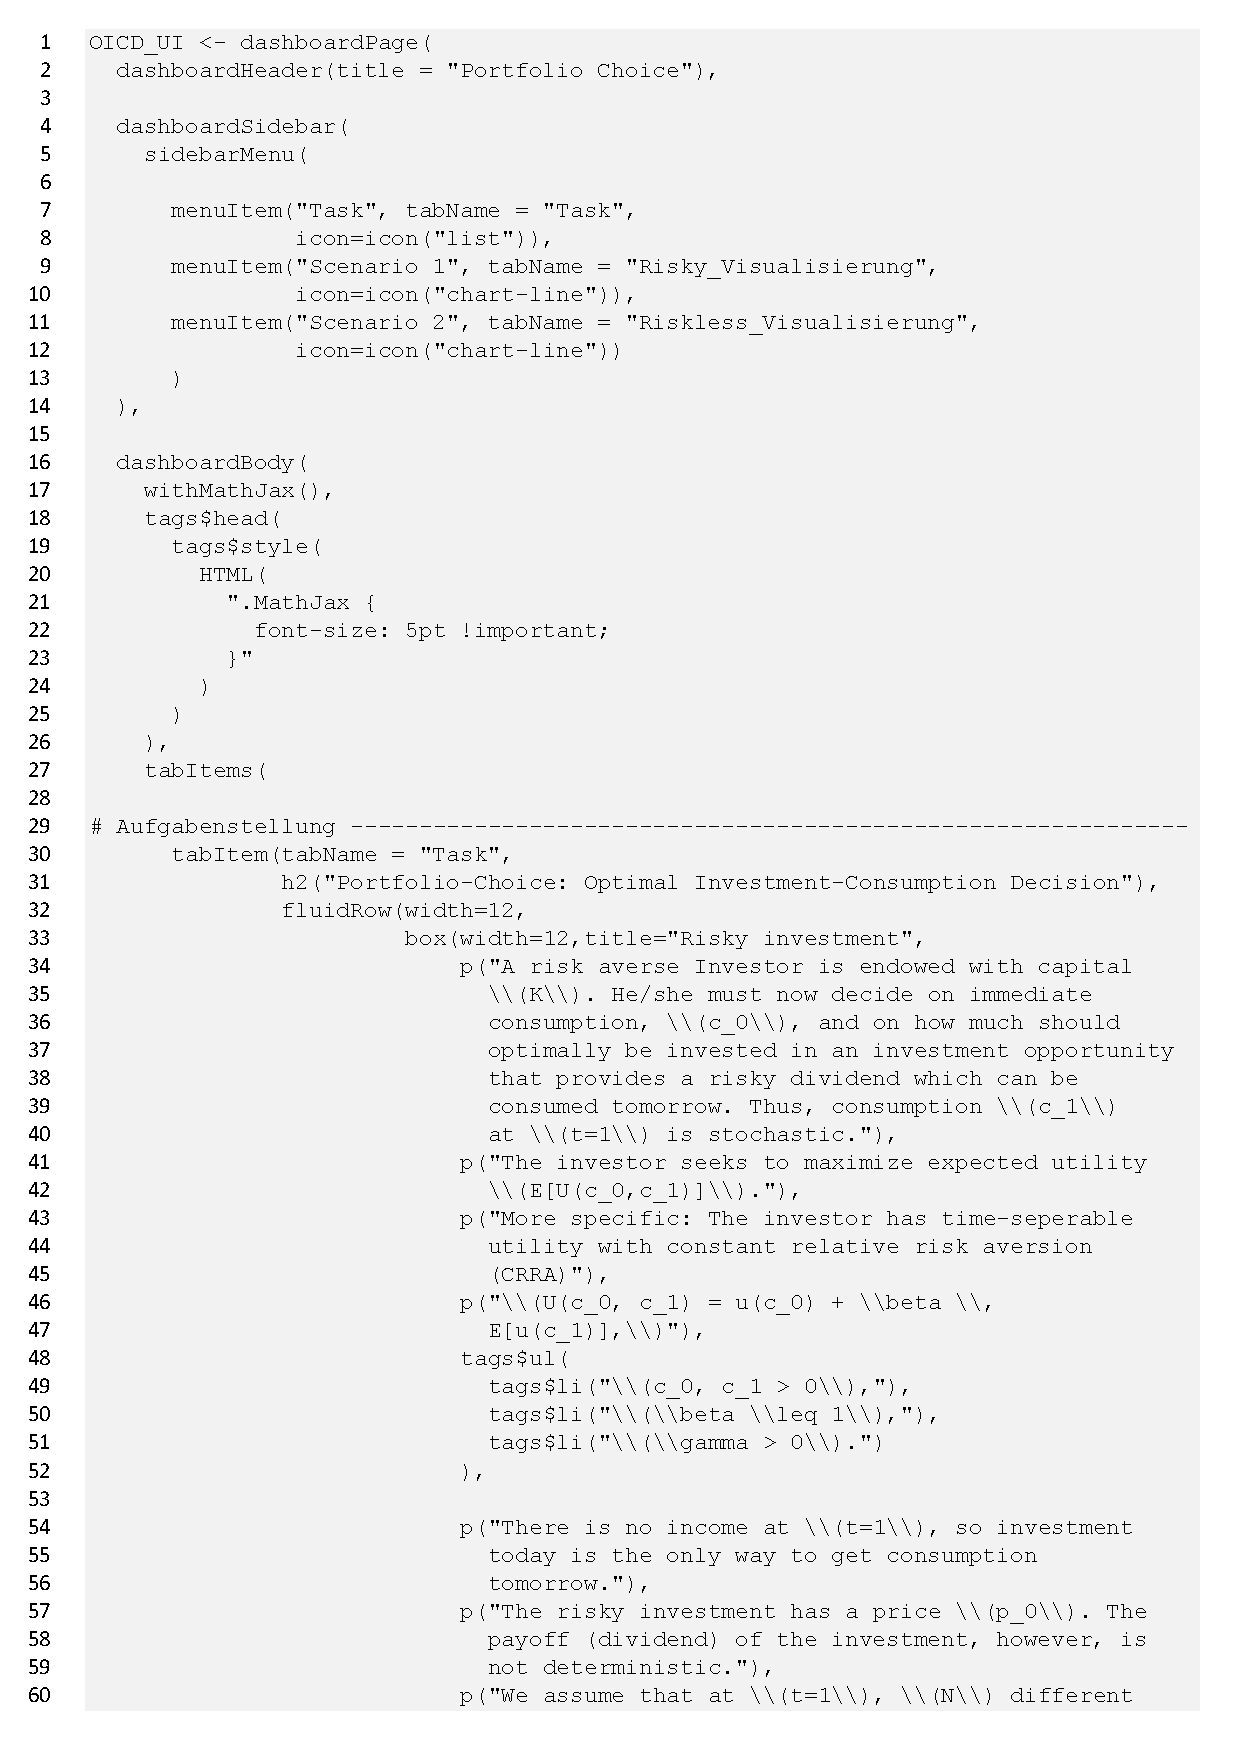
\includegraphics[scale=0.75, page = 1]{files/UI.pdf}
    \newpage
    \includegraphics[scale=0.75, page = 2]{files/UI.pdf}
    \newpage
    \includegraphics[scale=0.75, page = 3]{files/UI.pdf}
    \newpage
    \includegraphics[scale=0.75, page = 4]{files/UI.pdf}
    \newpage
    \includegraphics[scale=0.75, page = 5]{files/UI.pdf}
\end{center}



\hypertarget{Server function}{} \subsection*{Server Function}

\addcontentsline{toc}{subsection}{Server Function}
\begin{center}
    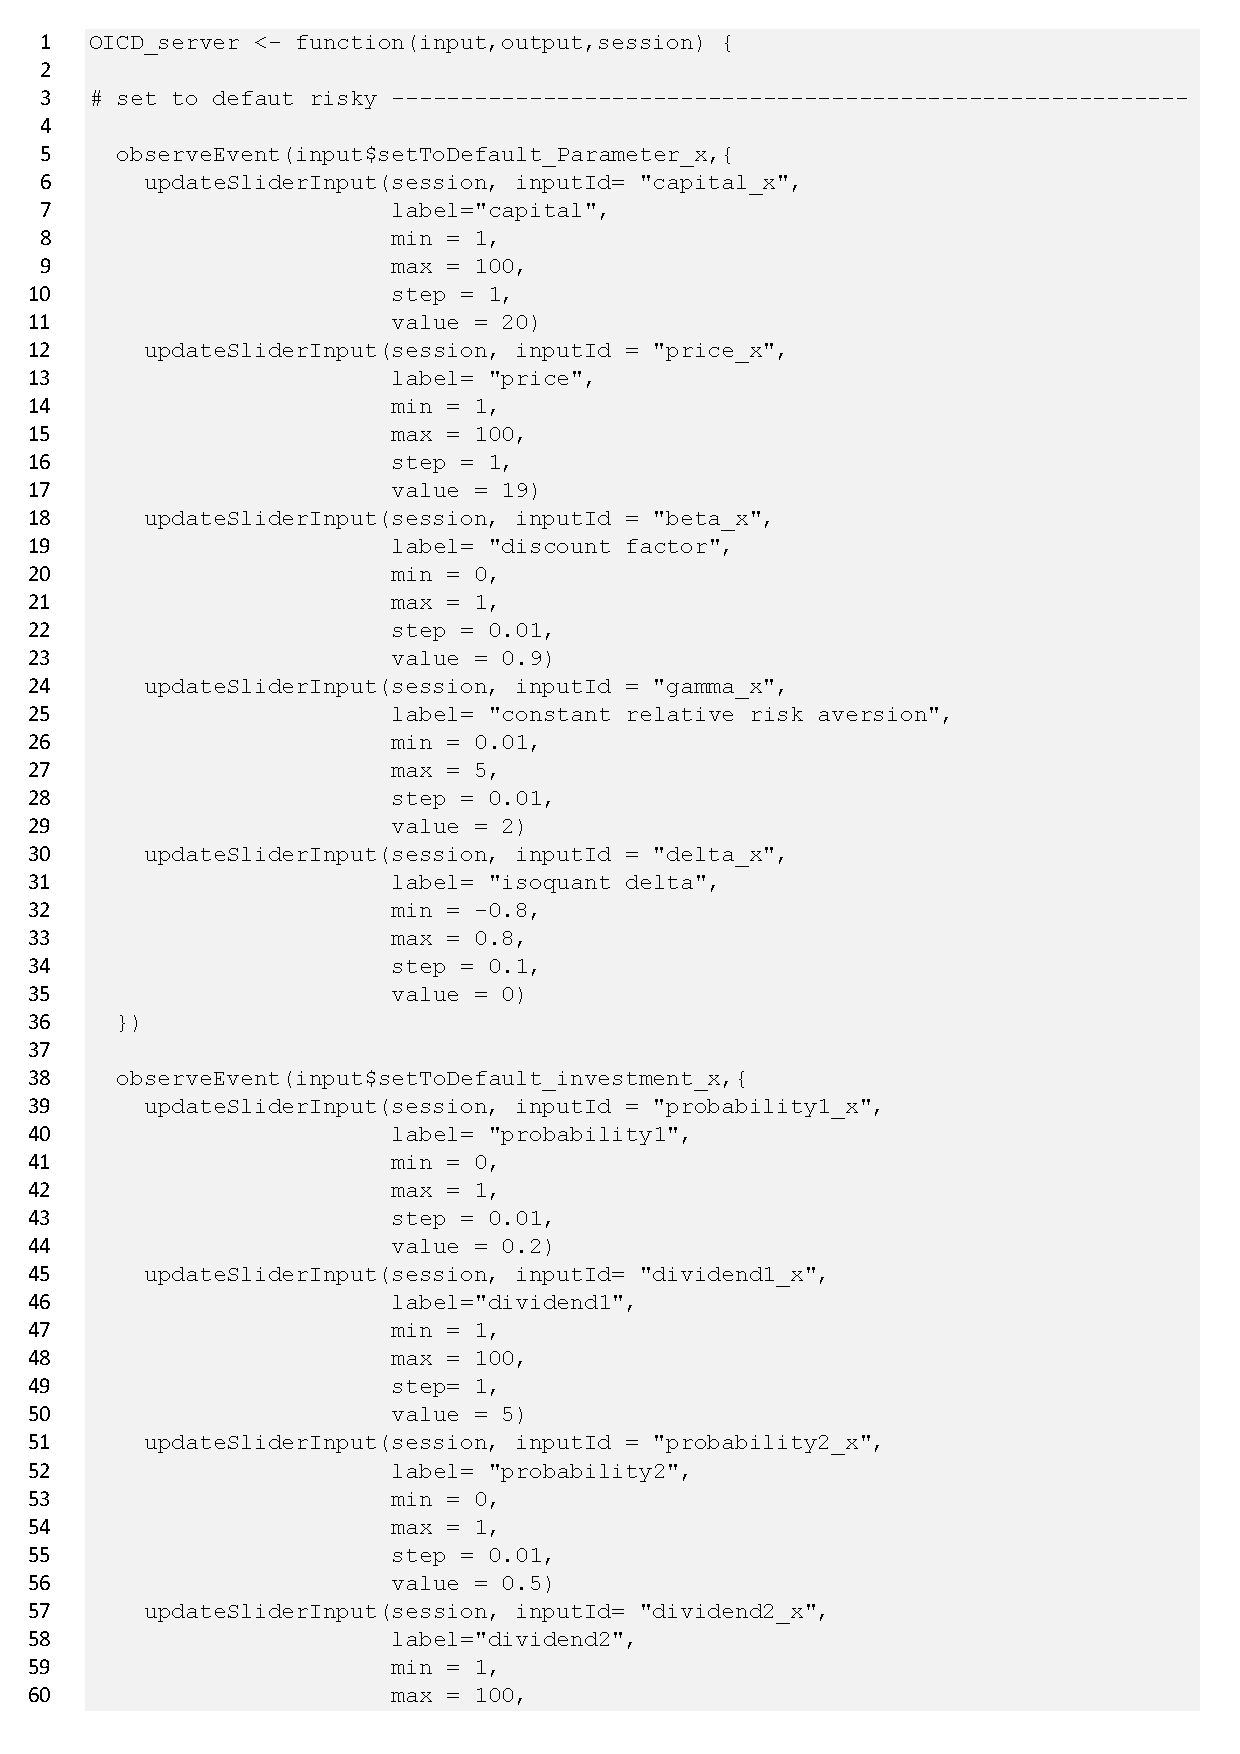
\includegraphics[scale=0.75, page = 1]{files/SERVER.pdf}
    \newpage
    \includegraphics[scale=0.75, page = 2]{files/SERVER.pdf}
    \newpage
    \includegraphics[scale=0.75, page = 3]{files/SERVER.pdf}
    \newpage
    \includegraphics[scale=0.75, page = 4]{files/SERVER.pdf}
    \newpage
    \includegraphics[scale=0.75, page = 5]{files/SERVER.pdf}
    \newpage
    \includegraphics[scale=0.75, page = 6]{files/SERVER.pdf}
    \newpage
    \includegraphics[scale=0.75, page = 7]{files/SERVER.pdf}
    \newpage
    \includegraphics[scale=0.75, page = 8]{files/SERVER.pdf}
    \newpage
    \includegraphics[scale=0.75, page = 9]{files/SERVER.pdf}
    \newpage
    \includegraphics[scale=0.75, page = 10]{files/SERVER.pdf}
    \newpage
    \includegraphics[scale=0.75, page = 11]{files/SERVER.pdf}
    \newpage
    \includegraphics[scale=0.75, page = 12]{files/SERVER.pdf}
    \newpage
    \includegraphics[scale=0.75, page = 13]{files/SERVER.pdf}
    \newpage
    \includegraphics[scale=0.75, page = 14]{files/SERVER.pdf}
    \newpage
    \includegraphics[scale=0.75, page = 15]{files/SERVER.pdf}
    \newpage
    \includegraphics[scale=0.75, page = 16]{files/SERVER.pdf}
    \newpage
    \includegraphics[scale=0.75, page = 17]{files/SERVER.pdf}
\end{center}


\hypertarget{call function}{} \subsection*{Call Function}
\addcontentsline{toc}{subsection}{Call Function}
\begin{center}
    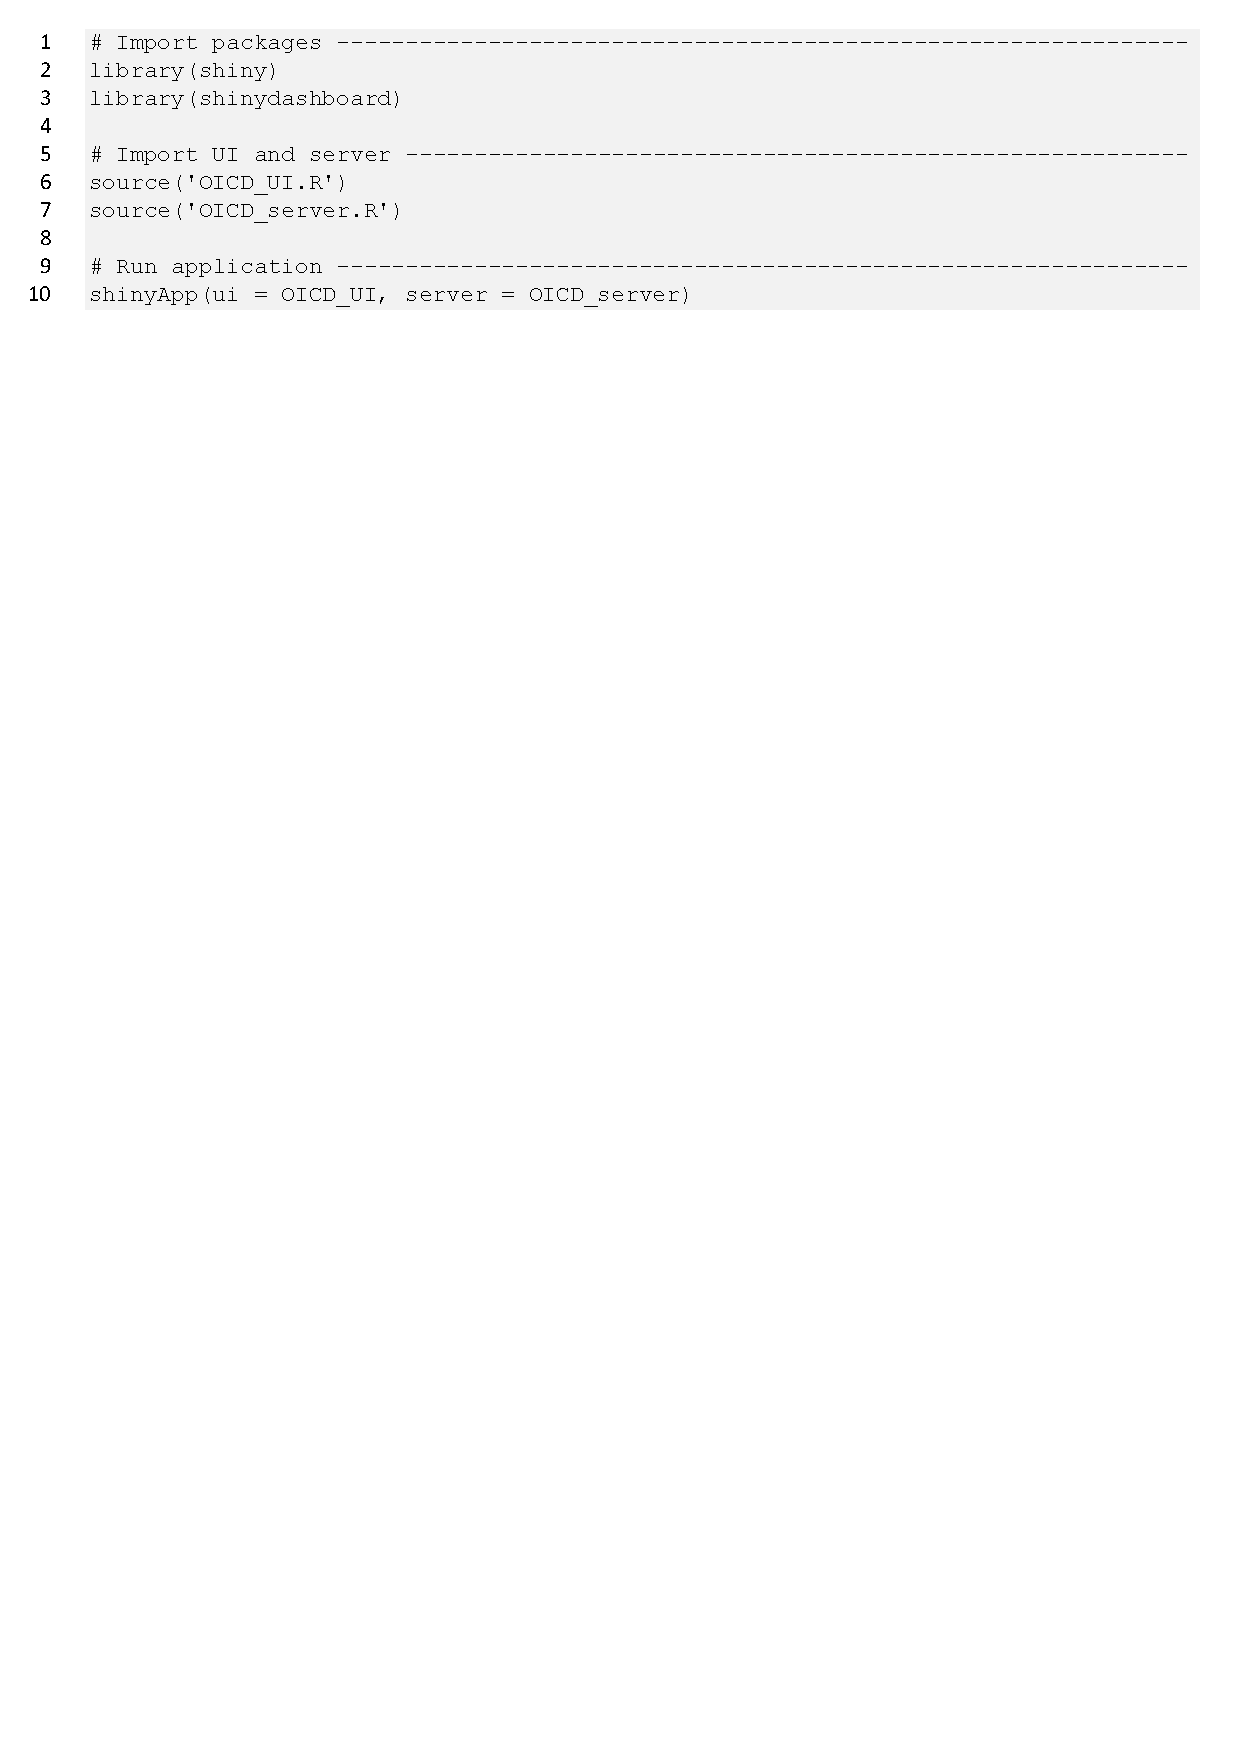
\includegraphics[scale=0.75, page = 1]{files/RUN.pdf}
\end{center}



\end{document}